\documentclass[a4j,10pt]{jsarticle}

%================================================================
% Include required packages
\usepackage[dvipdfmx]{graphicx}
\usepackage{ascmac,setspace}
\usepackage{cite}
\usepackage[normalem]{ulem}
\usepackage{fancybox}
%================================================================
% Original command definition
\def\vctr#1{\mbox{\boldmath $#1$}}
\newcommand{\bbn}[2]{\frac{{\rm {\rm d}} #1}{{\rm {\rm d}} #2}}
\newcommand{\henbbn}[2]{\frac{\partial #1}{\partial #2}}
\usepackage{amsmath, amssymb,amsfonts, amsthm}
%================================================================
% Re-define commands
\makeatletter % プリアンブルで定義開始
\renewcommand{\figurename}{Fig. }  % 表示文字列を"図"から"Figure"へ
\makeatother % プリアンブルで定義終了
%================================================================
\begin{document}
%================================================================
\title{解説:角速度と擬座標を用いた運動方程式}
\author{上村知也}
%================================================================
\setlength{\baselineskip}{3.8mm}	% 行間の設定
\maketitle
%\thispagestyle{empty}
%\pagestyle{empty}
\setstretch{1.0} % ページ全体の行間を設定
%================================================================
% \tableofcontents
% \newpage
%================================================================
\section{はじめに}
3次元空間内の角速度$\omega$は,3次元ベクトルで表せるが,これを積分しても姿勢を表すオイラー角にはならない.
そもそも,角速度は何らかの座標の時間微分として表すことができない.
これはなぜか,そしてそのような場合にラグランジュの運動方程式はどのように表されるのか考えてみよう.

\section{準備:すぐに積分できる微分方程式}

\subsection{全微分型の微分方程式}

角速度の議論を行う前にまず,積分関数が簡単に求められる微分方程式について考えるところから始めよう.
\begin{align}
    F(x,y){\rm d} x + G(x,y){\rm d} y=0
    \label{eq:zenbibun}
\end{align}
という形の微分方程式を全微分型の方程式と呼び,解は$\phi(x,y) = c$の形で与えられる.この方程式について詳しく見ていく.

\subsubsection*{ポテンシャル関数が存在すること}
ある関数$P, Q$がスカラーポテンシャル関数$\phi(x,y)$の偏微分で表されるとしよう.すなわち,
\begin{subequations}
    \begin{align}
        P(x,y) &= \frac{\partial \phi(x,y)}{\partial x}\\
        Q(x,y) &= \frac{\partial \phi(x,y)}{\partial y}
    \end{align}
\end{subequations}
とする.このとき,
\begin{align}
    \frac{\partial P}{\partial y} = \frac{\partial Q}{\partial x}
\end{align}
が成立する.$(x,y)$空間内にポテンシャル$\phi$に由来するベクトル場$(P,Q)$が存在すると考えるとイメージがつきやすい.

逆に,$\partial P/\partial y = \partial Q /\partial x$が成立するとしよう.このとき,
\begin{align}
    \phi(x,y) = \int_{\pi_0}^x P(x,y){\rm d} x + \int_{y_0}^y Q(\pi_0,y){\rm d} y
\end{align}
と定義すると,
\begin{align*}
    \frac{\partial \phi}{\partial x} = P(x,y)
\end{align*}
と
\begin{align*}
    \frac{\partial \phi}{\partial y}&=\int_{\pi_0}^x \frac{\partial P}{\partial y}{\rm d} x + Q(\pi_0,y)\\
    &=\int_{\pi_0}^x \frac{\partial Q}{\partial x}dx + Q(\pi_0,y)\\
    &= Q(x,y) - Q(\pi_0, y) + Q(\pi_0,y)\\
    &= Q(x,y)
\end{align*}
となり,$\phi$が確かにポテンシャル関数になっていることが確認される.

以上から,2次元ベクトル場$(P,Q)$がポテンシャル$\phi(x,y)$を持つための必要十分条件は$\partial P/\partial y - \partial Q /\partial x=0$が成立することである(ベクトル解析の言葉を使って,${\mathrm{rot}(P,Q)=0}$としてもよい).
言い換えると,偏微分が入れ替え可能であること,すなわち
\begin{align}
    \frac{\partial}{\partial y}\frac{\partial \phi}{\partial x}=\frac{\partial}{\partial x}\frac{\partial \phi}{\partial y}
\end{align}
が成立することが,ポテンシャル関数が存在することの必要十分条件である.このとき積分が経路に依存しない(Fig.~\ref{fig:integral_path}).

\begin{figure}
    \centering
    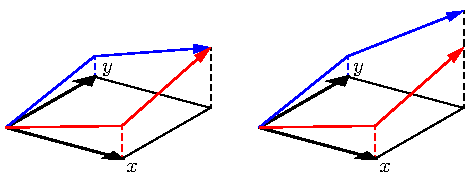
\includegraphics{integral_path.pdf}
    \caption{積分が経路に依存する場合とそうでない場合.左の場合,赤い経路と青い経路の最終到達点は同じであるが,右の場合は異なる点にたどり着く.左の場合が積分可能であり,積分が一意に定められる.}
    \label{fig:integral_path}
\end{figure}

以上から,全微分型の方程式\eqref{eq:zenbibun}の解は,ポテンシャル関数$\phi(x,y)=c$となる($c$は任意定数).

\subsection{一般化した全微分型の方程式}
上記を一般化する.$k,l=1,...,n$のすべての値に対して
\begin{align}
    \frac{\partial P_k}{\partial q_l} = \frac{\partial P_l}{\partial q_k}
\end{align}
が成立するとき,ポテンシャル関数$\phi(q_1,...,q_n)$が存在する.

全微分型の方程式
\begin{align}
    P_1 {\rm d} q_1 + P_2 {\rm d} q_2 + \cdots + P_n {\rm d} q_n=0
\end{align}
の解はポテンシャル関数$\phi(q_1,...,q_n)=c$で与えられる($c$は任意定数).
このような状況を,積分関数の存在が簡単に示せることから,\textbf{直ちに積分できる}と呼ぶことにしよう.

\section{真の座標と擬座標}
ここからは力学の問題を考える.
一般化座標$q_1,...,q_n$で表される系におけるラグランジュの運動方程式は
\begin{align}
    \bbn{}{t}\left(\frac{\partial T}{\partial \dot{q}_i}\right)-\frac{\partial T}{\partial q_i}=Q_i
    \label{eq:Lagrange_equation}
\end{align}
で与えられる.ここで,$T$は運動エネルギー,$Q_i$は一般化力である.ここでは保存力も$Q_i$に含めている.

速度$\omega_1,...,\omega_n$を,一般化座標$\dot{q}_1,...,\dot{q}_n$の一次結合で定義する:
\begin{align}
    \omega_i = a_{i1}\dot{q}_1 + a_{i2}\dot{q}_2+\cdots+a_{in}\dot{q}_n
    \label{eq:omega_definition}
\end{align}
ただし,$a_{ik}$は$q_1,...,q_n$の与えられた関数である(定数ではない).
上記の定義では,$\omega_i$は何らかの位置の時間微分としては定義されていない.
この新しい``速度''に対応する``位置''と呼べる関数$\pi_i$が存在すると仮定しよう(もしかするとそのような関数はないかもしれない!).
このとき,${\rm d} \pi_i$を微分${\rm d} q_1, ... ,{\rm d} q_n$の一次結合で
\begin{align}
    {\rm d}\pi_i = a_{i1}{\rm d} q_1 + a_{i2}{\rm d} q_2 + \cdots + a_{in}{\rm d} q_n
    \label{eq:derivative_of_pi}
\end{align}
と表す.$a_{ik}$は先ほどと同じ関数である.

ある$i$について,もし
\begin{align}
    \frac{\partial a_{ik}}{\partial q_l}=\frac{\partial a_{il}}{\partial q_k}
\end{align}
が成立するならば,\eqref{eq:derivative_of_pi}は全微分型の方程式であり,その解$\pi_i$は\textbf{直ちに積分できる}(ポテンシャル関数を求めればよい)ことになる.このような$\pi_i$を\textbf{真の座標}と呼ぶ.
この場合,$\omega_i$は正しく$\pi_i$の時間微分として与えられることになる.

\begin{itembox}{注意}
「ポテンシャル関数」と書いたが,エネルギーを求めるわけではない!速度を積分して位置を求める問題であることを失念してはならない.
\end{itembox}

ここで,
\begin{align}
    \henbbn{a_{ik}}{q_l}\neq\henbbn{a_{il}}{q_k}
\end{align}
となる場合を考えてみる.積分の順番によって結果が変わる場合である.
この場合には,${\rm d} \pi_1,...,{\rm d} \pi_n$は$\pi_1,...,\pi_n$の微分にはならない.このような量${\rm d} \pi_1,...{\rm d} \pi_n$を\textbf{擬座標の微分}と呼ぶ.
すなわち,速度を積分した量としての``位置''を明確な座標として定義できない.

\subsection{角速度が積分できないこと}
積分できない速度など,存在するのだろうか?答えはYesである.
例えば剛体の角速度は積分できない.
すなわち,角速度を積分することで姿勢を表すオイラー角やクォータニオンを得ることはできない.
無理やり積分を行うとして,剛体の姿勢は積分の経路に依存してしまうからである.

例えば,ある剛体を$y$軸と$z$軸まわりにそれぞれ90 degずつ回転させるという操作を考えよう.
初めに$z$軸まわりに回転させ,のちに$y$軸まわりに回転させた場合をFig.~\ref{fig:rotation}Aに示す.
これに対して,順序を反転させて先に$y$軸まわりに回転させた場合をFig.\ref{fig:rotation}~Bに示す.
結果として,2つの場合で剛体は異なる姿勢になっていることが確認できる.

\begin{figure}
    \centering
    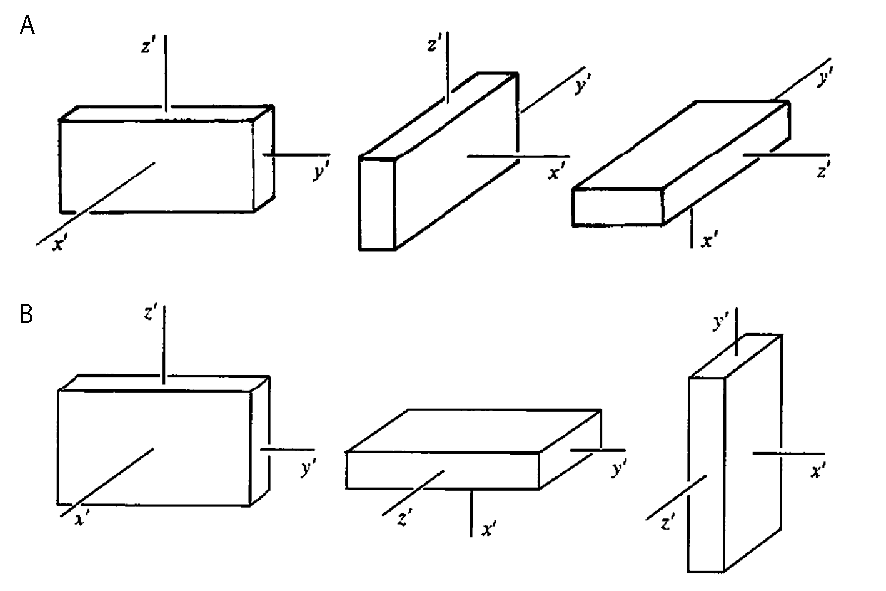
\includegraphics[width=120mm]{rotation.pdf}
    \caption{(A) $z$軸まわりの回転を行ったのち,$y$軸まわりの回転を行う場合.(B) $y$軸まわりの回転を行ったのち,$z$軸周りの回転を行う場合.図は\cite{Goldstein}から抜粋.}
    \label{fig:rotation}
\end{figure}

\section{擬座標でのラグランジュ方程式}

$r$番目の(擬)座標$\pi_r, \omega_r$についての運動方程式を,ラグランジュの運動方程式\eqref{eq:Lagrange_equation}から座標変換することで求めよう.

\subsection*{一般化力の変換}

一般化速度$\dot{q}_i$を速度$\omega_1,...,\omega_n$で表すと
\begin{align}
    \dot{q}_i=b_{i1}\omega_1+\cdots+b_{in}\omega_n
\end{align}
となる.$i=1,...,n$の$n$本の\eqref{eq:Lagrange_equation}にそれぞれ$b_{ir}$をかけて,和をとると
\begin{align}
    \sum_{i=1}^n b_{ir}\left\lbrace \bbn{}{t}\left(\henbbn{T}{\dot{q}_i}\right)-\henbbn{T}{q_i}\right\rbrace = \sum_{i=1}^n b_{ir}Q_i
    \label{eq:original_EOM}
\end{align}
任意の無限小変位$(\delta \pi_1,...,\delta \pi_n)$において外力が系にする仕事を$\delta W = F_1\delta \pi_1+\cdots+F_n\delta \pi_n$とすると,$F_r=\sum_{i} b_{ir}Q_i$が新しい座標系における「一般化力」となり,\eqref{eq:original_EOM}から
\begin{align}
    \sum_{i=1}^n b_{ir}\left\lbrace \frac{{\rm d}}{dt}\left(\frac{\partial T}{\partial \dot{q}_i}\right)-\frac{\partial T}{\partial q_i}\right\rbrace = F_r
    \label{eq:EOM_newGeneralizedForce}
\end{align}
を得る.

\subsection*{運動エネルギーの書き換え}

運動エネルギーも新しい速度の定義で書き直そう.
\begin{align*}
    T(q_1,...,q_n,\dot{q}_1,...,\dot{q}_n)=\bar{T}(q_1,...,q_n,\omega_1,...,\omega_n)
\end{align*}
としたとき
\begin{align*}
    \frac{\partial T}{\partial \dot{q}_i}=\sum_{k} a_{k i}\frac{\partial \bar{T}}{\partial \omega_k}
\end{align*}
となり,ラグランジュ方程式\eqref{eq:EOM_newGeneralizedForce}は
\begin{align}
    \sum_{i} b_{ir}\left\lbrace \sum_{k} a_{k i}\bbn{}{t}\left(\frac{\partial \bar{T}}{\partial \omega_k }\right)+ \sum_{k }\frac{\partial \bar{T}}{\partial \omega_k }\bbn{a_{k i}}{t} -\frac{\partial T}{\partial q_i}\right\rbrace = F_r
    \label{eq:EOM_newKineticEnergy}
\end{align}
と書き直される.

\subsection*{係数の整理}
ここで,\footnote{インデックス記号がややこしくなるので,総和に関する記号はアルファベットではなく$\#$を用いた.初めて見ると驚くかもしれないが,あえてこのようにした.}
\begin{align*}
    \omega_i   &= a_{i1}\dot{q}_1 + \cdots + a_{in}\dot{q}_n\\
                &=\quad  a_{i1}(b_{11}\omega_1+\cdots+b_{1i}\omega_i+\cdots+b_{1n}\omega_n)\\
                &\quad + a_{i2}(b_{21}\omega_1+\cdots+b_{2i}\omega_i+\cdots+b_{2n}\omega_n)\\
                &\quad\quad \vdots\\
                &\quad + a_{in}(b_{n1}\omega_1+\cdots+b_{ni}\omega_i+\cdots+b_{nn}\omega_n)\\
                &=\sum_\# a_{i\#}b_{\# 1}\omega_1 + \cdots + \sum_\# a_{i\#}b_{\# i}\omega_i + \cdots + \sum_\# a_{i\#}b_{\# n}\omega_n\\
                &=0\cdot\omega_1+\cdots+1\cdot\omega_i+\cdots+0\cdot\omega_n
\end{align*}
であるから,
\begin{align*}
    \sum_\# a_{i\#}b_{\# j}=\begin{cases}
    1 & i = j\\
    0 & i \neq j
    \end{cases}
\end{align*}
となる.これをラグランジュ方程式\eqref{eq:EOM_newKineticEnergy}に代入すると,$\bbn{}{t}(\henbbn{\bar{T}}{\omega_k})$の項は$k=r$のみが残り,
\begin{align}
    \bbn{}{t}\left(\henbbn{\bar{T}}{\omega_r}\right)+\sum_i\sum_k b_{ir}\bbn{a_{ik}}{t}\henbbn{\bar{T}}{\omega_k}-\sum_i b_{ir}\henbbn{T}{q_i}=F_r
\end{align}
となる.
さらに,
\begin{align*}
    \bbn{a_{ik}}{t} = \sum_\# \henbbn{a_{ik}}{q_\#}\dot{q}_\#
\end{align*}
を用いて,
\begin{align}
    \bbn{}{t}\left(\henbbn{\bar{T}}{\omega_r}\right)+\sum_i\sum_k\sum_\# b_{ir}\henbbn{\bar{T}}{\omega_k}\dot{q}_\# \henbbn{a_{ik}}{q_\#}-\sum_i b_{ir}\henbbn{T}{q_i}=F_r
    \label{eq:EOM_arrangedCoefficinets}
\end{align}
を得る.

\subsection*{位置に関係する項}
残るは$\henbbn{T}{q_i}$の項のみである.
$\bar{T}$は$q_1,...,q_n$と$\omega_1,...,\omega_n$の関数である.チェインルールから
\begin{align*}
    \henbbn{T}{q_i} &= \henbbn{\bar{T}}{q_i}+\henbbn{\bar{T}}{\omega_1}\henbbn{\omega_1}{q_i} + \henbbn{\bar{T}}{\omega_2}\henbbn{\omega_2}{q_i} \cdots +\henbbn{\bar{T}}{\omega_n}\henbbn{\omega_1}{q_n}\\
    &= \henbbn{\bar{T}}{q_i} + \sum_k \henbbn{\bar{T}}{\omega_k}\henbbn{\omega_k}{q_i}
\end{align*}
である.さらに速度$\omega_i$の定義\eqref{eq:omega_definition}から,
\begin{align*}
    \henbbn{\omega_k}{q_i}=
    \sum_\#\henbbn{a_{k\#}}{q_i}\dot{q}_\#
\end{align*}
となるので,
\begin{align*}
    \henbbn{T}{q_i} =\henbbn{\bar{T}}{q_i} + \sum_k \sum_\# \henbbn{\bar{T}}{\omega_k}\henbbn{a_{k\#}}{q_i}\dot{q}_\#
\end{align*}
を得る.
したがってラグランジュ方程式\eqref{eq:EOM_arrangedCoefficinets}は
\begin{align}
    \bbn{}{t}\left(\henbbn{\bar{T}}{\omega_r}\right)+\sum_i\sum_k\sum_\# b_{ir}\henbbn{\bar{T}}{\omega_k}\dot{q}_\# \left(\henbbn{a_{ik}}{q_\#} - \henbbn{a_{k\#}}{q_i}\right)-\sum_i b_{ir}\henbbn{\bar{T}}{q_i}=F_r
    \label{eq:EOM_position_changed}
\end{align}
もし$\pi_r$が真の座標であれば,左辺の最後の項
\begin{align*}
    \sum_i b_{ir}\henbbn{\bar{T}}{q_i} = \sum_i b_{ir}\henbbn{\bar{T}}{q_i}\henbbn{q_i}{\pi_r} = \henbbn{\bar{T}}{\pi_r}
\end{align*}
が成り立つ.
$\pi_r$が真の座標かどうかに関わらず,この項を$\partial{\bar{T}}/\partial{\pi_r}$と書くことにしよう.

また,
\begin{align}
    \sum_k\sum_\# b_{ir}b_{\# l} \left(\henbbn{a_{ik}}{q_\#} - \henbbn{a_{k\#}}{q_i}\right)
\end{align}
は考えている力学系の性質や運動とは無関係であり,これを$\gamma_{rkl}$と表すことにする.このとき,\eqref{eq:EOM_position_changed}は
\begin{align}
    \bbn{}{t}\left(\henbbn{\bar{T}}{\omega_r}\right)+\sum_k\sum_l \gamma_{rkl}\henbbn{\bar{T}}{\omega_k} - \sum_i b_{ir}\henbbn{\bar{T}}{q_i}=F_r
    \label{eq:EOM_quasiCoordinate}
\end{align}
となる.これが擬座標で表された運動方程式である.

\subsection*{真の座標ならどうなるか}
$\pi_r$が真の座標であれば,
\begin{align*}
    \henbbn{a_{ik}}{q_\#} - \henbbn{a_{k\#}}{q_i} = 0
\end{align*}
が成立するので,運動方程式\eqref{eq:EOM_quasiCoordinate}は
\begin{align}
    \bbn{}{t}\left(\henbbn{\bar{T}}{\omega_r}\right) - \sum_i b_{ir}\henbbn{\bar{T}}{q_i}=F_r
\end{align}
となり,普通のラグランジュの運動方程式と一致する.

\section{角速度を用いた運動方程式}
剛体が固定した一点$O$のまわりに自由に回転する.
物体の姿勢は,物体に固定された座標$Oxyz$の位置を,空間に固定した軸$OXYZ$に関して定めるオイラー角$(\theta, \phi, \psi)$で表される.
物体の任意の変位$(\delta\theta, \delta\phi, \delta\psi)$が,それぞれ$O_x$, $O_y$, $O_z$の周りの微小回転$\delta\pi_1, \delta\pi_2$, $\delta\pi_3$の合成値と同等とする.
$\omega_1$, $\omega_2$, $\omega_3$を各瞬間における物体の角速度の軸$Oxyz$のまわりの成分とする.
このとき,${\rm d}\pi_1$, ${\rm d}\pi_2$, ${\rm d}\pi_3$はそれぞれ速度$\omega_1$, $\omega_2$, $\omega_3$に対応する擬座標の成分である\footnote{繰り返すが,オイラー角$(\theta, \phi, \psi)$と擬座標$(\pi_1, \pi_2, \pi_3)$は異なることに注意しよう.}.
このとき,運動方程式は\eqref{eq:EOM_quasiCoordinate}から
\begin{subequations}
    \begin{align}
        \bbn{}{t}\left(\henbbn{\bar{T}}{\omega_1}\right) - \left(\omega_3\henbbn{\bar{T}}{\omega_2}- \omega_2\henbbn{\bar{T}}{\omega_3}\right)- \henbbn{\bar{T}}{\pi_1} = \tau_1\\
        \bbn{}{t}\left(\henbbn{\bar{T}}{\omega_2}\right) - \left(\omega_1\henbbn{\bar{T}}{\omega_3}- \omega_3\henbbn{\bar{T}}{\omega_1}\right)- \henbbn{\bar{T}}{\pi_2} = \tau_2\\
        \bbn{}{t}\left(\henbbn{\bar{T}}{\omega_3}\right) - \left(\omega_2\henbbn{\bar{T}}{\omega_1}- \omega_1\henbbn{\bar{T}}{\omega_2}\right)- \henbbn{\bar{T}}{\pi_3} = \tau_3
    \end{align}
\end{subequations}
となる.ただし,$\bar{T}$は$\omega_1, \omega_2, \omega_3, \theta, \phi, \psi$で表された物体の運動エネルギーであり,
$\tau_1, \tau_2, \tau_3$はそれぞれ軸$Ox$, $Oy$, $Oz$のまわりの物体に働く外力のモーメントである.
なお,$\partial \bar{T}/\partial\pi_r$は
\begin{align*}
    \henbbn{\bar{T}}{\pi_r} = \henbbn{\bar{T}}{\theta}\henbbn{\theta}{\pi_r} + \henbbn{\bar{T}}{\phi}\henbbn{\phi}{\pi_r} +\henbbn{\bar{T}}{\psi}\henbbn{\psi}{\pi_r}=0
\end{align*}
である.なぜなら運動エネルギーは角速度$\omega_1, \omega_2, \omega_3$のみで決まるから.

結局,回転の運動方程式は,擬座標$\pi_r$を用いずに
\begin{subequations}
    \begin{align}
        \bbn{}{t}\left(\henbbn{\bar{T}}{\omega_1}\right) - \left(\omega_3\henbbn{\bar{T}}{\omega_2}- \omega_2\henbbn{\bar{T}}{\omega_3}\right) = \tau_1\\
        \bbn{}{t}\left(\henbbn{\bar{T}}{\omega_2}\right) - \left(\omega_1\henbbn{\bar{T}}{\omega_3}- \omega_3\henbbn{\bar{T}}{\omega_1}\right) = \tau_2\\
        \bbn{}{t}\left(\henbbn{\bar{T}}{\omega_3}\right) - \left(\omega_2\henbbn{\bar{T}}{\omega_1}- \omega_1\henbbn{\bar{T}}{\omega_2}\right) = \tau_3
    \end{align}
\end{subequations}
と表せる.これはオイラーの運動方程式と呼ばれる.

%================================================================
\begin{thebibliography}{9}
    \bibitem{ODE} 笠原,微分方程式の基礎,朝倉書店,1982.
    \bibitem{Goldstein} Goldstein, 古典力学(上),吉岡書店,2006.
    \bibitem{Whitekker} Whittaker,解析力学〈上〉,講談社,1977.
\end{thebibliography}
\end{document}